\chapter{序論}\label{abst}
\section{背景と目的}
本文を書いていく.引用するときはciteを使う->\cite{cite_1}.
citeの文字列はdocument.txtの参考文献の文字列と合わせる.
すると自動的に番号を振ってくれる.

段落分けする場合はこのように空行を挟む.

画像を張る場合は以下のように記述する.

\begin{figure}[htbp]
  \begin{center}
    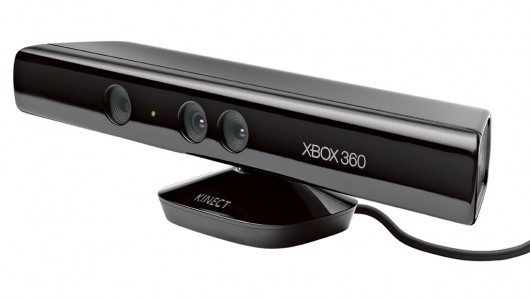
\includegraphics[clip,width=7.0cm]{./images/Kinect.jpg}
    \caption{Kinect}
    \label{fig:Kinect}
  \end{center}
\end{figure}

図ooと文中で用いる場合はrefを使用する->図\ref{fig:Kinect}.
図のlabelとrefの文字列を合わせることで自動的に番号を振ってくれる.
includegraphicsの./images/ファイル名を変更することで表示する画像を変更できる.
使用できる画像は.jpgと.pngのみ.

\section{論文構成}
論文構成を書いていく.
